\chapter{आणविक पादप-शरीरक्रिया और प्रतिबल-अनुक्रियाएँ}\label{ch:b3:plant-molecular-physiology}

किसी अँधेरी अलमारी में उगा सेम का कोई अंकुर पीली, दुबली-पतली चीज़ होता
है: कोई लंबा सफ़ेद तना, ऊपर कोई अंकुश, दो मुड़े पीले पत्ते। उसे किसी
खिड़की पर रखिए और दिन भर में उसने लंबा होना छोड़ दिया है, अपना अंकुश
सीधा कर लिया है, अपने पत्ते फैला और हरे कर लिए हैं --- यानी उन्हीं जीनों
से कोई दूसरा जीव। वह ऊर्जा की प्रतीक्षा नहीं कर रहा था; वह सूचना की
प्रतीक्षा कर रहा था। किसी एक प्रोटीन से अवशोषित कोई लाल फ़ोटॉन उसे बता
देता है कि वह प्रकाश तक पहुँच गया; लाल और दूर-लाल का अनुपात उसे बताता है
कि ऊपर किसी पड़ोसी का पत्ता है या नहीं; रात की लंबाई उसे मौसम बताती है;
उसकी जड़ों के जल-विभव की कोई गिरावट, हवा का कोई स्पर्श, उसके पत्ते पर
बैठे किसी जीवाणु का फ्लैजेलिन --- हर एक किसी ग्राही से पकड़ा जाता है,
किसी रासायनिक संकेत में बदला जाता है, और इसका उत्तर इस बदलाव से दिया
जाता है कि कौन-से जीन अभिव्यक्त हों और कौन-सी कोशिकाएँ बढ़ें। कोई पौधा
अपने पर्यावरण से भाग नहीं सकता; उसे उसे पढ़ना और अपने को फिर से गढ़ना
पड़ता है। यह अध्याय उसी पढ़ने के बारे में है: प्रकाश-ग्राही, \omterm{def:b3:endocrinology:hormone}{हॉर्मोन} और
वे आणविक पैमाने पर कैसे काम करते हैं, सूखे, नमक, ठंड तथा ताप की
अनुक्रियाएँ, और वह दो-परती प्रतिरक्षा-तंत्र जो पौधों ने बिना किसी एक भी
चलती कोशिका के विकसित किया।

\section{प्रकाश पढ़ना}

\begin{definition}[प्रकाश-ग्राही]\label{def:b3:plant-molecular-physiology:photoreceptors}
\index{फ़ाइटोक्रोम}\index{क्रिप्टोक्रोम}\index{फ़ोटोट्रोपिन}\index{प्रकाश-आकारजनन}\index{पीतन}
पौधे प्रकाश तीन प्रोटीन-कुलों से भाँपते हैं, और उनमें से कोई भी
पर्णहरित नहीं है। \emph{फ़ाइटोक्रोम} ऐसे द्विलक हैं जिनका बिलिन वर्णक
लाल प्रकाश (\qty{660}{nm}) से निष्क्रिय \emph{Pr} रूप से सक्रिय
\emph{Pfr} में और दूर-लाल (\qty{730}{nm}) से वापस बदल जाता है; Pfr
केंद्रक में चला जाता है और अनुलेखन कारकों के किसी कुल, यानी PIF, को
अपघटन के लिए चिह्नित कर देता है, जिससे प्रकाश में उगने के परिवर्धन के
जीन छूट जाते हैं; और अँधेरे में Pfr धीरे-धीरे पलट जाता है।
\emph{क्रिप्टोक्रोम} (नीला, \qty{450}{nm}) DNA-मरम्मत एंज़ाइमों से
संबंधित फ़्लेवोप्रोटीन हैं, जो अ-पीतन, वह घड़ी और पुष्पन नियंत्रित करते
हैं; और \emph{फ़ोटोट्रोपिन} (नीला) ऐसी झिल्ली-काइनेज़ हैं जो प्रकाश की
ओर झुकना, रंध्रों का खुलना और हरितलवकों का चलना संचालित करती हैं।
अँधेरे में कोई अंकुर \emph{पीतित} होता है --- लंबा बीजपत्रोपरिक, बंद
बीजपत्र, कोई पर्णहरित नहीं, और सारे संसाधन सतह तक पहुँचने में लगे हुए;
प्रकाश उसे \emph{प्रकाश-आकारजनन} पर स्विच कर देता है, और वह स्विच
Pfr तथा क्रिप्टोक्रोम द्वारा किसी एक ही दमनकारी संकुल (COP1) को
निष्क्रिय करने से चलता है, जो अँधेरे में प्रकाश-कार्यक्रम के अनुलेखन
कारक नष्ट कर देता है। इस तरह प्रकाश दो बार पढ़ा जाता है: ऊर्जा के रूप
में, हरितलवक द्वारा, और संकेत के रूप में, उन ग्राहियों द्वारा जो दस लाख
गुना छोटे फ़ोटॉन-फ्लक्स के प्रति संवेदी हैं।
\end{definition}

\begin{proposition}[फ़ाइटोक्रोम का प्रकाश-साम्य]\label{prop:b3:plant-molecular-physiology:photoequilibrium}
\index{प्रकाश-साम्य}\index{लाल:दूर-लाल अनुपात}\index{छाया-परिहार}
लगातार प्रकाश में Pr और Pfr तब तक आपस में बदलते रहते हैं जब तक दोनों
प्रकाश-परिवर्तन दरें संतुलित न हो जाएँ: $k_{1}$ को Pr $\to$ Pfr की दर
(जो लाल फ्लक्स के समानुपाती है) और $k_{2}$ को Pfr $\to$ Pr की
(जो दूर-लाल फ्लक्स के समानुपाती है, जमा लाल से थोड़ी, जिसे Pfr भी
अवशोषित करता है) लेने पर, सक्रिय रूप का अंश है
\[
\varphi = \frac{[\text{Pfr}]}{[\text{Pfr}] + [\text{Pr}]} = \frac{k_{1}}{k_{1} + k_{2}},
\]
जो कुल फ्लक्स से स्वतंत्र है और केवल उस प्रकाश के \emph{\omterm{prop:b3:plant-molecular-physiology:photoequilibrium}{लाल:दूर-लाल
अनुपात}} $\zeta$ से तय होता है। शुद्ध लाल $\varphi \approx 0.87$ देता है
(Pfr भी कुछ लाल अवशोषित करता है), शुद्ध दूर-लाल $0.03$; खुला दिन,
$\zeta \approx
1.15$, लगभग $0.55$ देता है, और किसी पर्ण-वितान के नीचे का प्रकाश, जिसके
पर्णहरित ने लाल निकाल लिया और दूर-लाल जाने दिया, $\zeta \approx 0.2$
और $\varphi \approx 0.2$ रखता है। कोई पौधा अपने $\varphi$ को पड़ोसियों
की उपस्थिति की तरह पढ़ता है: कोई कम मान \emph{छाया-परिहार} संलक्षण छेड़
देता है --- लंबे तने, उठे पत्ते, जल्दी पुष्पन, कम शाखन --- उन्हीं PIF
के ज़रिए जिन्हें Pfr अब नष्ट नहीं करता। किसी किसान की सघन बुवाई
छाया-परिहारियों की कोई दौड़ है; और हरित क्रांति के बौने गेहूँ, जो उस
संकेत के प्रति असंवेदी हैं, बची हुई वृद्धि दाने में लगा देते हैं।
\end{proposition}
\begin{proof}
$\mathrm{d}[\text{Pfr}]/\mathrm{d}t = k_{1}[\text{Pr}] - k_{2}[\text{Pfr}]$,
जिसमें $[\text{Pr}] + [\text{Pfr}] = P$ नियत हो, स्थायी अवस्था पर
$k_{1}(P - [\text{Pfr}]) = k_{2}[\text{Pfr}]$ देता है, जिससे $\varphi = k_{1}/
(k_{1} + k_{2})$। दोनों दरें आपाती फ्लक्स के समानुपाती हैं, इसलिए
प्रकाश को मापक्रमित करने पर दोनों मापक्रमित होती हैं और $\varphi$
अपरिवर्तित रहता है; केवल वर्णक्रमी संघटन मायने रखता है। वह स्थायी अवस्था
दर $k_{1} + k_{2}$ से छू ली जाती है --- धूप में सेकंडों में, गोधूलि में
मिनटों में --- और Pfr का अँधेरे में पलटना, जिसका अर्ध-आयु काल घंटों का
है, तय करता है कि रात में क्या बचता है।
\end{proof}

\begin{omfigure}
\begin{tikzpicture}[every node/.style={font=\scriptsize}, >=stealth]
  \node[draw, very thick, omDef, fill=omDef!15, rounded corners, minimum width=1.6cm, minimum height=0.9cm] (pr) at (0,0) {Pr (निष्क्रिय)};
  \node[draw, very thick, omThm, fill=omThm!15, rounded corners, minimum width=1.6cm, minimum height=0.9cm] (pfr) at (4.2,0) {Pfr (सक्रिय)};
  \draw[->, very thick, red!70!black] (pr.north east) to[bend left=25] node[above] {लाल, \qty{660}{nm}} (pfr.north west);
  \draw[->, very thick, red!40!black] (pfr.south west) to[bend left=25] node[below] {दूर-लाल, \qty{730}{nm}} (pr.south east);
  \draw[->, thick, gray] (pfr.south) ++(0.5,-0.15) to[bend left=40] node[right, font=\tiny, gray] {अँधेरे में पलटाव, घंटे} ++(-0.3,-0.9);
  \draw[->, thick] (pfr.east) -- ++(1.0,0) node[right, align=left] {केंद्रक में:\\PIF अपघटित, COP1 बंद;\\प्रकाश-कार्यक्रम चालू};
  \begin{scope}[shift={(0,-4.6)}]
  \begin{axis}[
    width=0.55\linewidth, height=4.6cm,
    axis x line=bottom, axis y line=left,
    xmin=0, xmax=2.5, ymin=0, ymax=1,
    xlabel={लाल:दूर-लाल अनुपात $\zeta$}, ylabel={$\varphi = $ Pfr अंश},
    xlabel style={font=\scriptsize, at={(axis description cs:0.5,-0.15)}, anchor=north}, ylabel style={font=\scriptsize},
    tick label style={font=\scriptsize}, xtick={0.2,0.5,1.15,2}, xticklabels={0.2,0.5,1.15,2}, ytick={0.2,0.55,0.87},
    clip=false,
  ]
  \addplot[very thick, omDef, domain=0:2.5, samples=80] {0.87*x/(x+0.6)};
  \draw[dashed, gray] (axis cs:0.2,0) -- (axis cs:0.2,0.22) -- (axis cs:0,0.22);
  \draw[dashed, gray] (axis cs:1.15,0) -- (axis cs:1.15,0.57) -- (axis cs:0,0.57);
  \node[font=\tiny, anchor=west, align=left] at (axis cs:0.25,0.12) {किसी वितान के नीचे:\\छाया-परिहार};
  \node[font=\tiny, anchor=south west] at (axis cs:1.2,0.62) {खुला दिन};
  \node[font=\tiny, anchor=north west, omDef, align=left] at (axis cs:1.6,0.45) {कोई आनुभविक फिट,\\$\varphi \approx 0.87\,\zeta/(\zeta + 0.6)$};
  \end{axis}
  \end{scope}
\end{tikzpicture}

{\small \omterm{def:b3:plant-molecular-physiology:photoreceptors}{फ़ाइटोक्रोम} का स्विच। लाल प्रकाश सक्रिय रूप बनाता है, दूर-लाल
उसे मिटाता है, अँधेरा धीरे-धीरे उसे पलट देता है; और सक्रिय रूप का स्थायी
अंश उस प्रकाश के रंग-संतुलन पर निर्भर है, उसकी चमक पर नहीं, और इसी से
कोई अंकुर जानता है कि उसके ऊपर कोई पत्ता है।}
\end{omfigure}

\begin{proof}[प्रमाण-सामग्री]
बोर्थविक, हेंड्रिक्स और सहयोगियों (1952) ने सलाद के बीजों को छोटी कौंधें
दीं: लाल ने उन्हें अंकुरित कराया, उसके बाद दिए गए दूर-लाल ने उसे रद्द
कर दिया, फिर लाल ने उसे लौटा दिया, और ऐसे ही दर्जन भर बारी-बारी ---
यानी आख़िरी कौंध ने तय किया, जो किसी उत्क्रमणीय वर्णक का हस्ताक्षर है,
जिसे उन्होंने फिर (1959) किसी ऐसे नीले प्रोटीन के रूप में निकाला जो लाल
और दूर-लाल के तहत अपना अवशोषण-वर्णक्रम बदल देता था। बाद में दिखाया गया
कि अँधेरे में उगे अंकुर का पूरा कार्यक्रम किसी एक दमनकारी पर टँगा है:
जिन उत्परिवर्तियों में COP1 न हो वे पूरे अँधेरे में ऐसे विकसित होते हैं
मानो प्रकाश में हों, छोटे और हरे होने को तैयार, और फ़ाइटोक्रोम- तथा
क्रिप्टोक्रोम-रहित उत्परिवर्ती प्रकाश में भी पीतित बने रहते हैं।
\end{proof}

\begin{omfigure}
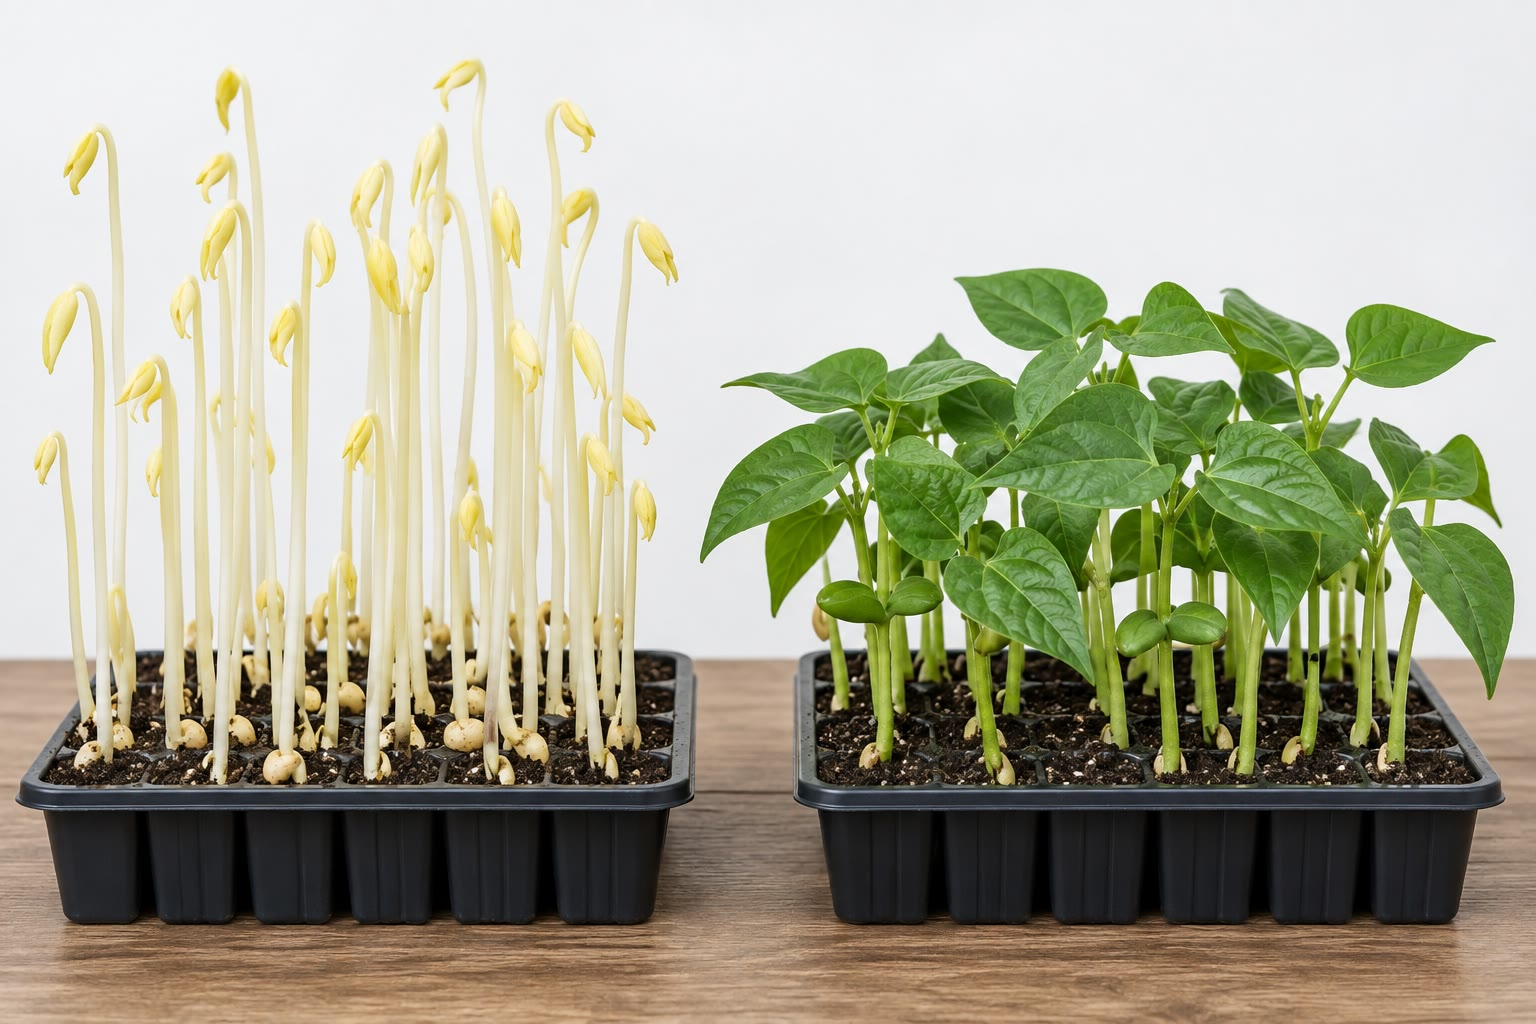
\includegraphics[width=0.56\linewidth]{images/book5/ai/b5-22-etiolated-seedlings.jpg}

{\small अँधेरे में और प्रकाश में उगे अंकुर: वही जीनोम, दो परिवर्धनी
कार्यक्रम, और वह अंतर \omterm{def:b3:plant-molecular-physiology:photoreceptors}{फ़ाइटोक्रोम} से अवशोषित किसी एक लाल फ़ोटॉन का है।}
\end{omfigure}

\section{आणविक पैमाने पर हॉर्मोन}

\begin{definition}[पादप हॉर्मोन और उनके ग्राही]\label{def:b3:plant-molecular-physiology:hormones}
\index{ऑक्सिन}\index{TIR1}\index{जिबरेलिन}\index{DELLA}\index{ऐब्सिसिक अम्ल}\index{एथिलीन}\index{साइटोकाइनिन}\index{ब्रैसिनोस्टेरॉइड}
वर्ष~1 के खंड ने बताया था कि पादप \omterm{def:b3:endocrinology:hormone}{हॉर्मोन} करते क्या हैं; यहाँ यह है कि
वे सुने कैसे जाते हैं। कई \emph{नियमित विनाश} से काम करते हैं।
\emph{ऑक्सिन} (इंडोल-3-ऐसीटिक अम्ल) F-बॉक्स प्रोटीन \emph{TIR1} से
बँधता है और उसे Aux/IAA दमनकारियों से चिपका देता है, जो फिर
यूबिक्विटिनित होकर प्रोटिएसोम से नष्ट कर दिए जाते हैं: और वे
ऑक्सिन-अनुक्रिया जीन, जिन्हें वे दबाए थे, मिनटों में चालू हो जाते हैं
--- यानी वह \omterm{def:b3:endocrinology:hormone}{हॉर्मोन} कोई आणविक गोंद है, और वह ग्राही उसी अपघटन-तंत्र का
हिस्सा। \emph{जिबरेलिन} वही काम वृद्धि के \emph{DELLA} दमनकारियों के
साथ करता है, अपने ग्राही GID1 के ज़रिए: और हरित क्रांति के बौने गेहूँ
तथा धान ऐसे DELLA प्रोटीन ढोते हैं जो नष्ट किए ही नहीं जा सकते, इसलिए
वे जितना भी जिबरेलिन बनाएँ, छोटे ही रहते हैं। \emph{जैस्मोनेट} वही तर्क
JAZ दमनकारियों के साथ चलाता है। \emph{ऐब्सिसिक अम्ल} (ABA), यानी सूखे
और प्रसुप्ति का \omterm{def:b3:endocrinology:hormone}{हॉर्मोन}, PYR/PYL ग्राहियों से बँधता है, जो फिर किसी
फ़ॉस्फ़ेटेज़ (PP2C) का निरोध करते हैं, जिससे कोई काइनेज़ (SnRK2) छूटती
है जो आयन-वाहिकाओं तथा अनुलेखन कारकों का फ़ॉस्फ़ोरिलन करती है --- यानी
कोई दोहरा ऋणात्मक, जो उस अनुक्रिया को तीखा बना देता है। \emph{एथिलीन},
जो कोई गैस है, ER झिल्ली के ताँबा-युक्त ऐसे ग्राहियों से बँधता है जो
उसकी अनुपस्थिति में उस अनुक्रिया को सक्रिय रूप से दबाए रखते हैं; और
बँधना उन्हें बंद कर देता है, जिससे पकने, जरण तथा प्रतिबल के जीन चालू हो
जाते हैं। \emph{साइटोकाइनिन} जीवाणुओं के दो-घटक तंत्रों जैसी
हिस्टिडीन-काइनेज़ ग्राहियों से काम करते हैं; और
\emph{ब्रैसिनोस्टेरॉइड}, यानी पौधे के स्टेरॉइड, किसी पृष्ठीय ग्राही
काइनेज़ से, न कि किसी \omterm{def:b3:endocrinology:hormone}{केंद्रकीय ग्राही} से --- यानी कहीं भी ऐसे अकेले
\omterm{def:b3:endocrinology:hormone}{स्टेरॉइड हॉर्मोन}, जो कोशिका-पृष्ठ पर सुने जाते हैं। पौधों के पास कोई
ग्रंथि नहीं: हर \omterm{def:b3:endocrinology:hormone}{हॉर्मोन} वहीं बनता है जहाँ उसकी ज़रूरत है, या विशिष्ट
वाहकों से ले जाया जाता है, और उसकी सांद्रता स्थानीय रूप से संश्लेषण,
संयुग्मन तथा विनाश से तय होती है।
\end{definition}

\begin{theorem}[ऑक्सिन का रसपरासरणी ध्रुवी परिवहन]\label{thm:b3:plant-molecular-physiology:auxin}
\index{ध्रुवी ऑक्सिन परिवहन}\index{PIN प्रोटीन}\index{ऋणायन-फँसाव}
इंडोल-3-ऐसीटिक अम्ल कोई दुर्बल अम्ल है, $\mathrm{p}K_{a} = 4.75$।
कोशिका-भित्ति के अवकाश में pH~$5.5$ पर उसका बड़ा अंश उदासीन IAAH है, जो
झिल्ली के आर-पार विसरित होता है; कोशिकाद्रव्य में pH~$7.2$ पर लगभग सारा
ऋणायन IAA$^{-}$ है, जो विसरण से निकल नहीं सकता। झिल्ली के आर-पार उदासीन
रूप के साम्य पर भीतर और बाहर के कुल \omterm{def:b3:plant-molecular-physiology:hormones}{ऑक्सिन} का अनुपात है
\[
\frac{[\text{IAA}]_{\text{भीतर}}}{[\text{IAA}]_{\text{बाहर}}}
= \frac{1 + 10^{\,\mathrm{pH}_{\text{भीतर}} - \mathrm{p}K_{a}}}{1 + 10^{\,\mathrm{pH}_{\text{बाहर}} - \mathrm{p}K_{a}}}
\approx \frac{283}{6.6} \approx 43 :
\]
यानी वह कोशिका \omterm{def:b3:plant-molecular-physiology:hormones}{ऑक्सिन} को चालीस गुना फँसा लेती है। वह केवल \emph{PIN}
बहिर्वाह वाहकों से निकल सकता है, और चूँकि हर कोशिका अपने PIN किसी एक
फलक पर रखती है --- तने में आधारी फलक पर --- चारों ओर से लिया गया \omterm{def:b3:plant-molecular-physiology:hormones}{ऑक्सिन}
सब नीचे से निकलता है, अगली कोशिका में घुसता है, और ऐसे ही: यानी एक ही
ध्रुवता वाली कोशिकाओं का कोई स्तंभ कोई ऐसी पट्टी है जो \omterm{def:b3:plant-molecular-physiology:hormones}{ऑक्सिन} को
प्ररोह-शिखर से जड़ तक लगभग \qty{1}{cm/h} पर ले जाती है, और PIN को फिर
से मोड़ देने से वह धारा मुड़ जाती है, और इसी से किसी तने के छायादार पक्ष
में अधिक \omterm{def:b3:plant-molecular-physiology:hormones}{ऑक्सिन} आ जाता है और वह तेज़ बढ़ता है।
\end{theorem}
\begin{proof}
हेंडरसन--हैसलबाल्क: $[\text{IAA}^{-}]/[\text{IAAH}] = 10^{\,\mathrm{pH}
- \mathrm{p}K_{a}}$, इसलिए कुल $= [\text{IAAH}](1 + 10^{\,\mathrm{pH} -
\mathrm{p}K_{a}})$। उदासीन रूप संतुलित होता है, $[\text{IAAH}]_{\text{भीतर}}
= [\text{IAAH}]_{\text{बाहर}}$; दोनों कुलों को भाग देने पर वह अनुपात
मिलता है, $(1 + 10^{2.45})/(1 + 10^{0.75}) = 283/6.6$। किसी एक फलक पर
PIN होने से उस ऋणायन का इकलौता निकास दिशात्मक है; $n$ कोशिकाओं का कोई
स्तंभ उस फ्लक्स को आगे सरका देता है, और नापा गया वेग, जो इन दूरियों पर
विसरण से एक कोटि ऊपर है, हर कोशिका-सीमा पर वाहक-मध्यस्थ बहिर्वाह का
वेग है। चोलोदनी--वेंट परिकल्पना (1920 का दशक), कि झुकना \omterm{def:b3:plant-molecular-physiology:hormones}{ऑक्सिन} के किसी
पार्श्व पुनर्वितरण के पीछे चलता है, जई के प्रांकुरचोलों में सीधे मापन से
और करवट लिटाई गई \emph{Arabidopsis} जड़ों में PIN के स्थानांतरण के
प्रतिबिंबन से पुष्ट हुई (2000 का दशक)।
\end{proof}

\begin{omfigure}
\begin{tikzpicture}[every node/.style={font=\scriptsize}, >=stealth]
  % three cells in a column
  \foreach \y in {0,-2.2,-4.4} {
    \draw[thick, omDef, fill=omDef!8] (0,\y) rectangle (3.2,\y-1.9);
    \draw[very thick, omThm] (0.6,\y-1.9) -- (2.6,\y-1.9);
    \node[right, font=\tiny] at (3.3,\y-0.4) {कोशिकाद्रव्य pH 7.2};
    \node[right, font=\tiny] at (3.3,\y-0.8) {IAA$^{-}$ फँसा};
    \draw[->, thick, omDef!70!black] (-0.6,\y-0.6) -- (0.4,\y-0.6); \node[left, font=\tiny] at (-0.6,\y-0.6) {IAAH भीतर};
    \draw[->, thick, omDef!70!black] (3.8,\y-1.3) -- (2.8,\y-1.3);
    \draw[->, very thick, omThm] (1.6,\y-1.5) -- (1.6,\y-2.35);
  }
  \node[left, align=right, font=\tiny] at (-0.6,-1.4) {भित्ति pH 5.5:\\\qty{15}{\%} IAAH,\\\qty{85}{\%} IAA$^{-}$};
  \node[omThm, right, font=\tiny] at (3.3,-2.05) {PIN बहिर्वाह वाहक, केवल आधारी फलक पर};
  \node[above] at (1.6,0.1) {प्ररोह-शिखर: ऑक्सिन का स्रोत};
  \node[below] at (1.6,-6.8) {जड़ की ओर, \qty{1}{cm/h}};
  \node[right, align=left] at (5.4,-3.6) {भीतर : बाहर $\approx 43 : 1$\\(ऋणायन का फँसाव)\\[3pt]निकास केवल PIN से,\\इसलिए वह स्तंभ कोई पट्टी है;\\PIN किसी पार्श्व फलक पर ले जाइए\\और वह धारा मुड़ जाती है};
\end{tikzpicture}

{\small \omterm{thm:b3:plant-molecular-physiology:auxin}{ध्रुवी ऑक्सिन परिवहन} का रसपरासरणी प्रतिरूप। वह अम्ल किसी भी फलक
से उदासीन अणु के रूप में घुसता है, कोशिकाद्रव्य के pH पर ऋणायन के रूप
में फँस जाता है, और केवल उन वाहकों से निकलता है जो उस कोशिका ने किसी एक
फलक पर रखे हैं --- इसलिए कोशिकाओं की कोई पंक्ति \omterm{def:b3:plant-molecular-physiology:hormones}{ऑक्सिन} को एक ही दिशा
में सरकाती है।}
\end{omfigure}

\begin{example}[गुरुत्वानुवर्तन और प्रकाशानुवर्तन]\label{ex:b3:plant-molecular-physiology:tropism}
किसी अंकुर को करवट लिटाइए। मूलगोप में, स्तंभिका कोशिकाओं के सघन
स्टार्च-भरे लवक मिनटों के भीतर नए निचले पक्ष पर बैठ जाते हैं; उन
कोशिकाओं के PIN3 वाहक निचले फलक पर चले जाते हैं; \omterm{def:b3:plant-molecular-physiology:hormones}{ऑक्सिन} उस जड़ के निचले
पार्श्व में अधिक बहने लगता है, जहाँ वह, जड़-कोशिकाओं के इष्टतम से ऊपर
होने के कारण, दीर्घन का \emph{निरोध} करता है, और वह जड़ नीचे की ओर मुड़
जाती है। प्ररोह में वही पार्श्व बहाव निचले पक्ष में दीर्घन को
\emph{बढ़ावा} देता है (प्ररोह-कोशिकाओं का इष्टतम ऊँचा है), और वह प्ररोह
ऊपर की ओर मुड़ जाता है। प्रकाशानुवर्तन: किसी प्ररोह के प्रकाशित पक्ष का
\omterm{def:b3:plant-molecular-physiology:photoreceptors}{फ़ोटोट्रोपिन} PIN की जगह बदल देता है, जिससे \omterm{def:b3:plant-molecular-physiology:hormones}{ऑक्सिन} छायादार पक्ष में जमा
हो जाता है, जो तेज़ बढ़ता है और उस प्ररोह को प्रकाश की ओर मोड़ देता है।
दोनों गतियाँ धीमी हैं --- घंटों की --- क्योंकि वे वृद्धि हैं, गति नहीं,
और दोनों उस ऊतक में अनुत्क्रमणीय हैं जो बढ़ चुका है। डार्विन (1880) ने
दिखाया कि किसी घास-अंकुर का शिखर प्रकाश भाँपता है और नीचे का क्षेत्र
झुकता है; वेंट (1928) ने उस प्रभाव को किसी कटे शिखर पर रखे ऐगार-गुटके
में इकट्ठा किया और दिखाया कि किसी शिरोच्छिन्न प्ररोह पर असममित रखा
कोई गुटका उसे झुका देता है: वह प्रभाव कोई विसरणशील पदार्थ था, जिसे फिर
\omterm{def:b3:plant-molecular-physiology:hormones}{ऑक्सिन} नाम दिया गया।
\end{example}

\section{जल, नमक, ठंड और ताप}

\begin{definition}[अजैविक प्रतिबल]\label{def:b3:plant-molecular-physiology:abiotic}
\index{सूखा-प्रतिबल}\index{परासरणी समायोजन}\index{लवण-प्रतिबल}\index{शीत-अभ्यस्तन}\index{ताप-आघात प्रोटीन}
कोई पौधा भाग नहीं सकता, इसलिए वह कठोर हो जाता है। \emph{सूखा}: जड़ों
में गिरता जल-विभव ABA का संश्लेषण छेड़ देता है; ABA मिनटों में रंध्र बंद
कर देता है, और दिनों में \emph{परासरणी समायोजन} के जीन चालू कर देता है
(प्रोलीन, शर्कराएँ और दूसरे संगत विलेय जमा होते हैं, जिससे उस कोशिका
का जल-विभव गिरता है और वह जल खींचती रहती है), उन डिहाइड्रिनों के जीन
जो प्रोटीन बचाते हैं, और छोटे पर्ण-क्षेत्रफल तथा गहरी जड़ के।
\emph{नमक} सूखा जमा विष है: सोडियम पोटैशियम वाहिकाओं से घुसता है और
पोटैशियम से स्पर्धा करता है; सहिष्णु पौधे उसे जड़ों से बाहर पंप कर देते
हैं (SOS पथ), रसधानियों में (NHX विनिमयक), या पत्ती-ग्रंथियों से
उत्सर्जित कर देते हैं, और उनका \emph{लवणोद्भिद} छोर समुद्री जल में जीता
है। \emph{ठंड}: शीतलन झिल्लियाँ कड़ी कर देता है और एंज़ाइम धीमी;
हिमीकरण कोशिकाओं से जल खींचकर बाह्यकोशिकीय बर्फ़ में ले जाता है और
उन्हें सुखा देता है। \emph{शीत-अभ्यस्तन} --- ठंडे दिनों का हफ़्ता ---
CBF अनुलेखन कारक प्रेरित करता है, जो झिल्ली को तरल रखते लिपिडों,
शर्कराओं, प्रति-हिम प्रोटीनों तथा डिहाइड्रिनों के सैकड़ों जीन चालू कर
देते हैं, और जो शीत राई अगस्त में \qty{-5}{\celsius} पर मर जाती वह
जनवरी में \qty{-30}{\celsius} झेल जाती है। \emph{ताप} प्रोटीन खोल देता
है; किसी बढ़त के मिनटों के भीतर कोई ताप-आघात कारक \emph{ताप-आघात
प्रोटीन} छोड़ देता है, यानी ऐसे सहायक जो उन्हें फिर वलित करते या ठिकाने
लगाते हैं, और वे वही कुल हैं जो हर जीव में हैं। \emph{बाढ़} जड़ों को
ऑक्सीजन से वंचित कर देती है; धान वायु-नलिकाएँ (वायूतक) बनाता है और
लंबा होकर अपने पत्ते जल के ऊपर रखता है, और वह संकेत \omterm{def:b3:plant-molecular-physiology:hormones}{एथिलीन} है, जो तब
जमा होता है जब वह जल में निकल नहीं पाता। इनमें से अनेक कार्यक्रम
अतिव्यापी हैं --- ABA, क्रियाशील ऑक्सीजन जातियाँ और कैल्सियम-स्पंद साझा
द्वितीय संदेशवाहक हैं --- और किसी एक प्रतिबल का अभ्यस्त कोई पौधा प्रायः
किसी दूसरे से भी कुछ हद तक सुरक्षित रहता है।
\end{definition}

\begin{proposition}[वाल्व के रूप में रंध्र]\label{prop:b3:plant-molecular-physiology:stomata}
\index{रंध्र}\index{द्वार कोशिका}\index{रंध्रीय चालकता}\index{जल-उपयोग दक्षता}
हर रंध्र-छिद्र को \emph{\omterm{prop:b3:plant-molecular-physiology:stomata}{द्वार कोशिकाओं}} की कोई जोड़ी घेरे रहती है; वह
छिद्र तब खुलता है जब वे पोटैशियम तथा ऋणायन भीतर लेती हैं (और शर्करा
बनाती हैं), फूलती हैं, और अलग झुक जाती हैं, और तब बंद होता है जब वे
उन्हें खो दें। नीला प्रकाश (\omterm{def:b3:plant-molecular-physiology:photoreceptors}{फ़ोटोट्रोपिन}), कम CO$_{2}$ और आर्द्रता उसे
खोलते हैं; अँधेरा, ऊँचा CO$_{2}$, सूखा और ABA उसे बंद करते हैं। ABA का
रास्ता: ग्राही $\to$ फ़ॉस्फ़ेटेज़ निरोधित $\to$ काइनेज़ सक्रिय $\to$
ऋणायन वाहिकाएँ (SLAC1) खुलीं $\to$ झिल्ली विध्रुवित $\to$ पोटैशियम
बाहरगामी वाहिकाओं से निकला $\to$ जल पीछे गया $\to$ वह छिद्र बंद, दस
मिनट में। वह छिद्र वही जगह है जहाँ पौधे का केंद्रीय सौदा होता है:
CO$_{2}$ भीतर और जलवाष्प बाहर, दोनों उसी एक छेद से विसरित होते हैं, और
चूँकि वाष्प की प्रवणता (भीतर \qty{100}{\%} आर्द्रता वाला कोई पत्ता
बनाम \qty{50}{\%} की हवा) CO$_{2}$ की प्रवणता (बाहर \qty{400}{ppm},
भीतर \qty{250}{}) से पचास गुना तीखी है, कोई पत्ता अपने स्थिर किए हर
कार्बन अणु के लिए कई सौ जल-अणु खो देता है। \emph{\omterm{prop:b3:plant-molecular-physiology:stomata}{रंध्रीय चालकता}}
$g_{s}$ दोनों फ्लक्स तय करती है: वाष्पोत्सर्जन $E = g_{s}\,\Delta w$ और
स्वांगीकरण $A = (g_{s}/1.6)\,\Delta c$ (CO$_{2}$ भारी होने के कारण
$1.6$ गुना धीरे विसरित होती है), इसलिए \emph{\omterm{prop:b3:plant-molecular-physiology:stomata}{जल-उपयोग दक्षता}}
$A/E = \Delta c/(1.6\,\Delta w)$ उन प्रवणताओं पर निर्भर है, इस पर नहीं
कि वह छिद्र कितना खुला है; छिद्र बंद करने से दोनों फ्लक्स साथ गिरते
हैं, और भीतरी CO$_{2}$ चढ़ाना (C$_{4}$ पौधे, जो उसे सांद्रित करते हैं)
या केवल रात में खोलना (CAM पौधे, ठंडी नम हवा में) वह ढंग है जिससे
रेगिस्तानी पौधे उस अनुपात को सुधारते हैं।
\end{proposition}
\begin{proof}
हर गैस के लिए उस छिद्र के आर-पार फ़िक का नियम, जिसमें वही ज्यामितीय
चालकता विसरण-गुणांकों के अनुपात से मापक्रमित हो,
$D_{\mathrm{H_2O}}/D_{\mathrm{CO_2}} = 1.6$; और दोनों फ्लक्स को भाग
देने पर $g_{s}$ कट जाती है। संख्याएँ: \qty{25}{\celsius} और
\qty{50}{\%} आर्द्रता पर हवा का $\Delta w \approx \qty{15}{mmol/mol}$,
$\Delta c \approx
\qty{150}{\micro mol/mol}$: $A/E = 150/(1.6\times\num{15000}) = 1/160$
--- यानी उन नरम परिस्थितियों में $160$ जल-अणु प्रति CO$_{2}$, और सूखी
हवा में $500$। ABA की क्रिया का क्रम पैच क्लैंप के तहत द्वार-कोशिका
प्रोटोप्लास्टों से निकाला गया, जिसमें वह ऋणायन धारा ABA के मिनट भर के
भीतर प्रकट होती थी और SLAC1-रहित उत्परिवर्ती बंद होने में विफल रहता था।
\end{proof}

\begin{omfigure}
\begin{tikzpicture}[every node/.style={font=\scriptsize}, >=stealth]
  % pore with two guard cells
  \begin{scope}[shift={(0,0)}]
    \fill[omProp!30] (0,0) ellipse (1.4 and 0.9);
    \fill[white] (0,0) ellipse (0.5 and 0.6);
    \draw[thick, omProp!80!black] (0,0) ellipse (1.4 and 0.9); \draw[thick, omProp!80!black] (0,0) ellipse (0.5 and 0.6);
    \node[below, font=\tiny] at (0,-1.0) {खुला: K$^{+}$, Cl$^{-}$, मैलेट भीतर, स्फीत};
    \draw[->, thick, omDef] (0,0.3) -- (0,1.5) node[above, font=\tiny] {H$_2$O बाहर, $E = g_{s}\Delta w$};
    \draw[->, thick, omThm] (0,1.5) ++(-1.0,0) -- ++(0,-1.2); \node[left, font=\tiny, omThm] at (-1.1,1.0) {CO$_2$ भीतर, $A = g_{s}\Delta c/1.6$};
  \end{scope}
  \begin{scope}[shift={(4.2,0)}]
    \fill[omProp!30] (0,0) ellipse (1.2 and 0.75);
    \draw[thick, omProp!80!black] (0,0) ellipse (1.2 and 0.75); \draw[very thick, omProp!80!black] (0,-0.5) -- (0,0.5);
    \node[below, font=\tiny] at (0,-0.9) {बंद: आयन गए, शिथिल};
  \end{scope}
  \draw[->, thick] (1.6,0) -- (2.8,0) node[midway, above, font=\tiny] {ABA, अँधेरा,};
  \node[font=\tiny] at (2.2,-0.25) {ऊँची CO$_2$};
  % ABA pathway chain
  \begin{scope}[shift={(7.0,1.7)}]
    \node[draw, rounded corners, fill=omDef!20, align=center, font=\tiny] (a) at (0,0) {ABA PYR/PYL\\से बँधता};
    \node[draw, rounded corners, fill=omThm!15, align=center, font=\tiny] (b) at (0,-0.9) {PP2C फ़ॉस्फ़ेटेज़\\निरोधित};
    \node[draw, rounded corners, fill=omMeth!25, align=center, font=\tiny] (c) at (0,-1.8) {SnRK2 काइनेज़\\सक्रिय};
    \node[draw, rounded corners, fill=omProp!25, align=center, font=\tiny] (d) at (0,-2.7) {SLAC1 ऋणायन वाहिका\\खुली: विध्रुवण};
    \node[draw, rounded corners, fill=omProp!25, align=center, font=\tiny] (e) at (0,-3.6) {K$^{+}$ बाहर, जल बाहर,\\छिद्र \qty{10}{min} में बंद};
    \draw[-|, thick] (a) -- (b); \draw[-|, thick] (b) -- (c); \draw[->, thick] (c) -- (d); \draw[->, thick] (d) -- (e);
    \node[right, font=\tiny, align=left] at (1.5,-0.9) {शृंखला में दो\\निरोध:\\कोई तीखा स्विच};
  \end{scope}
\end{tikzpicture}

{\small वह रंध्र और वह संकेत जो उसे बंद करता है। जल और कार्बन
डाइऑक्साइड वही छिद्र साझा करते हैं, इसलिए वह पौधा एक को दूसरे के बदले
उस दर पर बेचता है जो दोनों प्रवणताएँ तय करती हैं; और सूखे का \omterm{def:b3:endocrinology:hormone}{हॉर्मोन}
दो निरोधों की किसी शृंखला से उस वाल्व को बंद कर देता है, जिससे वह
अनुक्रिया स्विच जैसी हो जाती है।}
\end{omfigure}

\begin{omfigure}
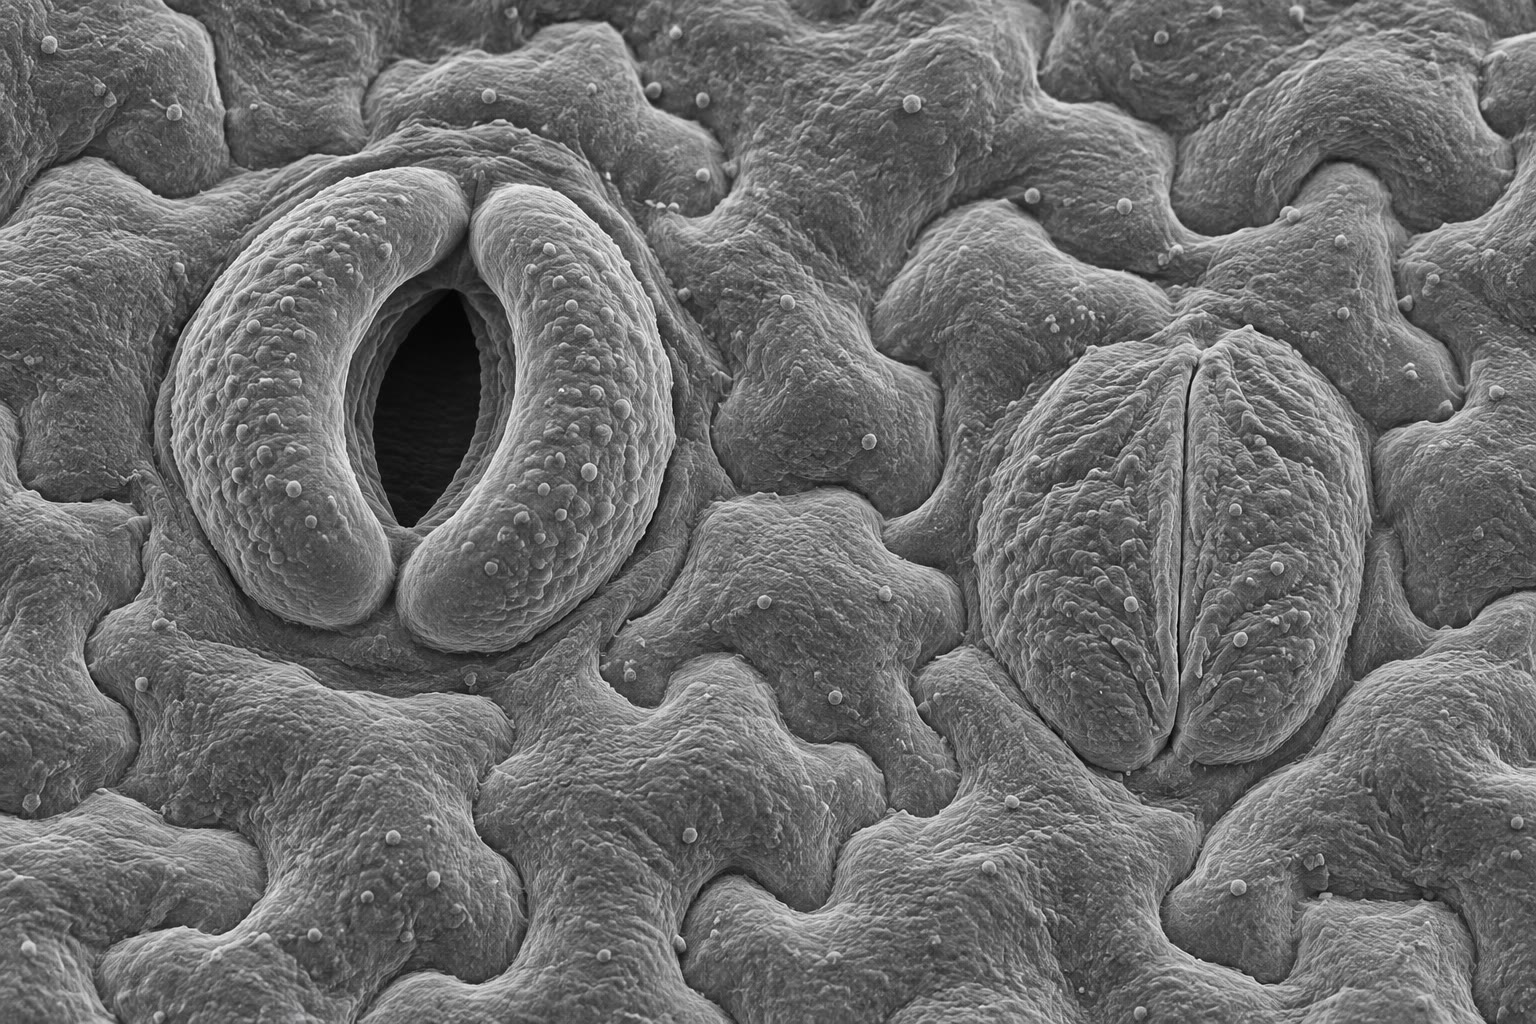
\includegraphics[width=0.46\linewidth]{images/book5/ai/b5-22-stomata-sem.jpg}\hspace{0.04\linewidth}
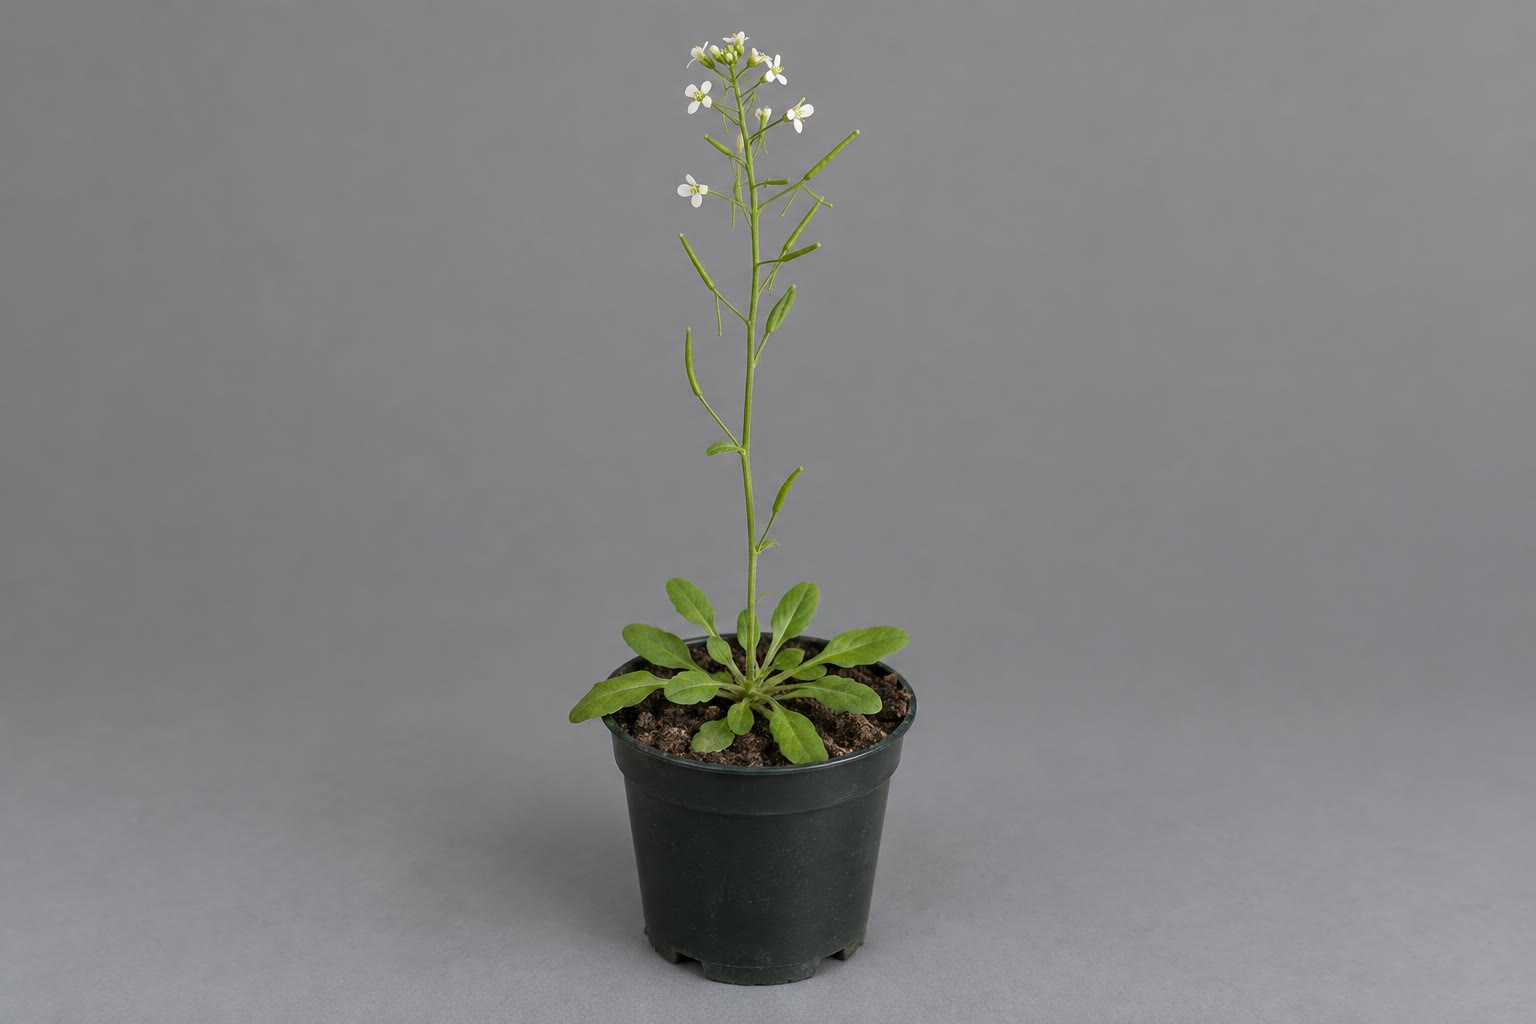
\includegraphics[width=0.46\linewidth]{images/book5/ai/b5-22-arabidopsis.jpg}

{\small बाएँ: किसी पत्ते के पृष्ठ पर रंध्र, हर छिद्र अपनी दो \omterm{prop:b3:plant-molecular-physiology:stomata}{द्वार
कोशिकाओं} के बीच, कुछ खुले और कुछ बंद। दाएँ: \emph{Arabidopsis
thaliana}, यानी छोटे जीनोम, छह-सप्ताह की पीढ़ी और एक लाख उत्परिवर्ती
वंशक्रमों वाला कोई सड़क-किनारे का खरपतवार, जिसमें इस अध्याय के अधिकांश
अणु खोजे गए।}
\end{omfigure}

\section{बिना प्रतिरक्षा-कोशिकाओं के प्रतिरक्षा}

\begin{definition}[पादप प्रतिरक्षा की दो परतें]\label{def:b3:plant-molecular-physiology:immunity}
\index{नमूना-छेड़ी प्रतिरक्षा}\index{कारक-छेड़ी प्रतिरक्षा}\index{NLR ग्राही}\index{अतिसंवेदी अनुक्रिया}\index{तंत्र-व्यापी अर्जित प्रतिरोध}\index{सैलिसिलिक अम्ल}\index{जैस्मोनिक अम्ल}
पौधे की हर कोशिका अपनी ही प्रतिरक्षा-कोशिका है। पहली परत,
\emph{नमूना-छेड़ी प्रतिरक्षा} (PTI), ऐसी पृष्ठीय ग्राही काइनेज़ काम
में लेती है जो सूक्ष्मजीवों के पूरे वर्गों में साझा अणु पहचानती हैं ---
FLS2 जीवाणु फ्लैजेलिन का 22-ऐमीनो-अम्ल टुकड़ा बाँधती है, दूसरी कवक
भित्तियों के काइटिन-टुकड़े --- और मिनटों के भीतर कैल्सियम-अंतर्वाह,
क्रियाशील ऑक्सीजन का कोई झोंका, काइनेज़-शृंखलाएँ, रंध्रों का बंद होना,
कैलोस से भित्ति का मोटा होना, और सैकड़ों रक्षा-जीनों का अनुलेखन छेड़
देती है; वह अधिकांश सूक्ष्मजीव रोक लेती है। जो रोगजनक सफल होते हैं वे
\emph{कारक} अंतःक्षिप्त करते हैं --- यानी ऐसे प्रोटीन जो PTI के घटक
अपंग कर दें --- और उनके विरुद्ध दूसरी परत, \emph{कारक-छेड़ी प्रतिरक्षा}
(ETI), कोशिका के भीतर \emph{NLR ग्राही} (न्यूक्लिओटाइड-बंधक,
ल्यूसीन-धनी पुनरावृत्ति) उतारती है, जिनमें हर एक किसी एक कारक को या
उसकी की हुई क्षति को पहचानता है, उसी जीन-दर-जीन जोड़ी में जिसका वर्णन
फ़्लोर ने अलसी के किट्ट में किया (1940 का दशक)। ETI, PTI से तेज़ तथा
प्रबल है और प्रायः \emph{अतिसंवेदी अनुक्रिया} में समाप्त होती है:
संक्रमित कोशिका और उसके पड़ोसी अपने को मार डालते हैं, और उस रोगजनक को
मरे ऊतक में चुन देते हैं --- यानी किसी प्रतिरोधी पत्ते पर वे छोटे भूरे
धब्बे। दोनों परतें ऐसे \omterm{def:b3:endocrinology:hormone}{हॉर्मोन} छोड़ती हैं जो वह चेतावनी ढोते हैं:
जीवपोषियों (जो जीवित कोशिकाओं पर पलते हैं) के विरुद्ध \emph{सैलिसिलिक
अम्ल}, जो पूरे पौधे में हफ़्तों के लिए \emph{तंत्र-व्यापी अर्जित
प्रतिरोध} छेड़ देता है; और मृतपोषियों (जो मारकर फिर खाते हैं) तथा
कुतरते कीटों के विरुद्ध \emph{जैस्मोनिक अम्ल} और \omterm{def:b3:plant-molecular-physiology:hormones}{एथिलीन}, जिसमें
वाष्पशील जैस्मोनेट पड़ोसी पौधों को चेताते हैं और उन कीटों के परजीविकाभ
खींचते हैं। वे दोनों \omterm{def:b3:endocrinology:hormone}{हॉर्मोन} एक-दूसरे का विरोध करते हैं, और कुछ रोगजनक
इसका फ़ायदा उठाते हैं: जो जीवाणु कोई जैस्मोनेट-नक़ल बनाता है वह उस
सैलिसिलेट-रक्षा को बंद कर देता है जो उसे रोक देती।
\end{definition}

\begin{omfigure}
\begin{tikzpicture}
\begin{axis}[
  width=0.78\linewidth, height=5.4cm,
  axis x line=bottom, axis y line=left,
  xmin=0, xmax=10, ymin=0, ymax=10,
  xlabel={वह होड़, बाएँ से दाएँ}, ylabel={रक्षा का आयाम},
  xlabel style={font=\small, at={(axis description cs:0.5,-0.08)}, anchor=north}, ylabel style={font=\small},
  xtick=\empty, ytick=\empty,
  clip=false,
]
\addplot[very thick, omDef] coordinates {(0,1) (1.5,5)};
\addplot[very thick, omThm] coordinates {(1.5,5) (3.2,1.8)};
\addplot[very thick, omDef] coordinates {(3.2,1.8) (4.8,8)};
\addplot[very thick, omThm] coordinates {(4.8,8) (6.4,2.2)};
\addplot[very thick, omDef] coordinates {(6.4,2.2) (8.0,8.6)};
\draw[dashed, gray] (axis cs:0,4) -- (axis cs:8.5,4); \node[font=\scriptsize, gray, anchor=west] at (axis cs:8.5,4) {प्रतिरोध की देहली};
\draw[dashed, gray] (axis cs:0,7.2) -- (axis cs:8.5,7.2); \node[font=\scriptsize, gray, anchor=west] at (axis cs:8.5,7.2) {अतिसंवेदी अनुक्रिया};
\node[font=\scriptsize, omDef, anchor=south west] at (axis cs:0.1,5.3) {PTI: ग्राही फ्लैजेलिन, काइटिन देखते हैं};
\node[font=\scriptsize, omThm, anchor=north, align=center] at (axis cs:3.2,1.6) {कारक अंतःक्षिप्त:\\PTI अपंग};
\node[font=\scriptsize, omDef, anchor=south, align=center] at (axis cs:4.8,8.2) {ETI: कोई NLR किसी\\कारक को पहचानता है};
\node[font=\scriptsize, omThm, anchor=north, align=center] at (axis cs:6.4,2.0) {कारक खोया या बदला:\\पहचान से बच निकला};
\node[font=\scriptsize, omDef, anchor=south, align=center] at (axis cs:8.0,8.8) {कोई नया NLR\\विकसित होता है};
\end{axis}
\end{tikzpicture}

{\small पादप--रोगजनक सहविकास की टेढ़ी चाल। पृष्ठीय ग्राही आम
सूक्ष्मजीवी अणुओं के विरुद्ध कोई रक्षा खड़ी करते हैं; रोगजनक ऐसे कारक
अंतःक्षिप्त करते हैं जो उसे दबा दें; पौधे उन कारकों के लिए
कोशिका-भीतरी ग्राही विकसित करते हैं; रोगजनक उन्हें झाड़ देते या बदल
देते हैं; और ऐसे ही, हर पग प्रतिरोध तथा विषाणुता के वे जीन छोड़ता जाता
है जिनका लेन-देन प्रजनक और रोगजनक अब भी करते हैं।}
\end{omfigure}

\begin{proof}[प्रमाण-सामग्री]
फ़्लोर (1940 का दशक) ने अलसी की किस्मों और किट्ट-प्रभेदों के संकरण किए
और पाया कि हर प्रभेद के प्रति प्रतिरोध पौधे के किसी एक प्रभावी जीन की
तरह अलग होता था, जिससे उस कवक में कोई एक अविषाणुता जीन मेल खाता था ---
यानी वही जीन-दर-जीन संबंध, जो पचास वर्षों तक अनसुलझा रहा, जब तक पहले
NLR जीन क्लोन न हुए (1994) और पहले कारक--ग्राही जोड़े एक-दूसरे को
बाँधते या एक-दूसरे की क्षति चिह्नित करते न दिखाए गए। गोमेज़-गोमेज़ और
बोलर (2000) ने फ्लैजेलिन के प्रति अंधा \emph{Arabidopsis} उत्परिवर्ती,
\emph{fls2}, पाया और दिखाया कि उसकी ग्राही काइनेज़ पेप्टाइड flg22 को
नैनोमोलर सांद्रता पर बाँधती थी और वह उत्परिवर्ती पत्तों पर छिड़के गए
जीवाणुओं के प्रति अधिक संवेद्य था पर उनमें अंतःक्षिप्त किए गए जीवाणुओं
के प्रति नहीं --- यानी वह ग्राही उस पृष्ठ और उन रंध्रों की चौकसी करता
है जिनसे जीवाणु घुसते हैं। रॉस (1961) ने किसी तंबाकू के पौधे के एक
पत्ते में कोई \omterm{def:b3:virology:virus}{विषाणु} टीका और हफ़्ता भर बाद बाकी पत्ते प्रतिरोधी पाए:
यानी \omterm{def:b3:plant-molecular-physiology:immunity}{तंत्र-व्यापी अर्जित प्रतिरोध}, जिसके लिए बाद में \omterm{def:b3:plant-molecular-physiology:immunity}{सैलिसिलिक अम्ल}
ज़रूरी दिखाया गया, जिसे वह पौधा उसी पथ से बनाता है जिससे ऐस्पिरिन का
जनक आता है।
\end{proof}

\begin{example}[पौधे की घड़ी और दिन की लंबाई]\label{ex:b3:plant-molecular-physiology:clock}
पौधे वैसी ही अभिकल्प की \omterm{def:b3:endocrinology:clock}{दैनिक घड़ी} रखते हैं जैसी प्राणियों की है, पर
असंबंधित पुर्ज़ों की: सुबह के कारक (CCA1, LHY) किसी शाम के जीन (TOC1)
को दबाते हैं, जिसका उत्पाद उन्हें दबाता है, और आगे के पाश उसे लगातार
प्रकाश में भी कोई मज़बूत 24-घंटे का चक्र बना देते हैं, जो सूरज से घंटा
भर पहले रंध्र खोलकर और प्रकाश-संश्लेषण के जीन चालू करके भोर की
प्रत्याशा करता है। उस घड़ी का सबसे परिणामी निर्गम दिन की लंबाई का मापन
है। \emph{Arabidopsis} में, जो कोई दीर्घ-दिन पौधा है, वह घड़ी CONSTANS
प्रोटीन को देर दोपहर में जमा करा देती है; किसी लंबे दिन में वह दोपहर अब
भी प्रकाशित है, \omterm{def:b3:plant-molecular-physiology:photoreceptors}{फ़ाइटोक्रोम} तथा \omterm{def:b3:plant-molecular-physiology:photoreceptors}{क्रिप्टोक्रोम} उस प्रोटीन को स्थिर कर
देते हैं, और वह पत्ते में \emph{FT} चालू कर देता है; किसी छोटे दिन में
वह प्रोटीन अँधेरे में बनता है और नष्ट कर दिया जाता है। FT प्रोटीन, यानी
वह पुष्पजन जिसका पीछा कलम-प्रयोग चायलाख़्यान (1936) से करते आए थे,
फ्लोएम में प्ररोह-शीर्ष तक जाता है और वहाँ किसी साथी के साथ उस शीर्ष को
पत्ते बनाने से फूल बनाने पर बदल देता है। लघु-दिन पौधे (धान, सोयाबीन) वही
घड़ी उलटे चिह्न के साथ काम में लेते हैं। इस तरह कोई पौधा किसी भीतरी लय
की बाहरी प्रकाश से तुलना करके पंचांग पढ़ता है --- यानी वही ``बाह्य
संपात'' जो ब्यूनिंग ने 1936 में सुझाया था और जिसे आणविक आनुवंशिकी ने
सत्तर वर्ष बाद शब्दशः बना दिया।
\end{example}

\begin{remark}[खड़े रहकर सब कुछ बदलना]\label{rem:b3:plant-molecular-physiology:remark}
किसी बुरे पर्यावरण का प्राणी का उत्तर उसे छोड़ देना है; पौधे का उत्तर
कोई दूसरा पौधा बन जाना है। उसके पास प्रकाश के रंग तथा दिशा के, गुरुत्व
के खिंचाव के, अपनी मिट्टी के जल-विभव के, हवा के स्पर्श के और अपने
शत्रुओं के रसायन के ग्राही हैं; उसके \omterm{def:b3:endocrinology:hormone}{हॉर्मोन} दमनकारियों को नष्ट करके
काम करते हैं, ताकि कोई संकेत मिनटों में कोई कार्यक्रम बदल सके; और उसकी
हर कोशिका अपना ही संवेदक, अपना ही प्रतिरक्षा-तंत्र और, ज़रूरत पड़े तो,
अपना ही पुनर्जनन करता विभज्योतक है। जिन बौने गेहूँओं ने बढ़ती दुनिया
को खिलाया वे कोई ऐसा \omterm{def:b3:plant-molecular-physiology:hormones}{DELLA} प्रोटीन थे जो अपघटित नहीं किया जा सकता था;
और अगले दशकों की सूखा-सहिष्णु फ़सलें, बड़े हिस्से में, ABA ग्राहियों,
\omterm{prop:b3:plant-molecular-physiology:stomata}{रंध्रीय चालकता} और उस \omterm{prop:b3:plant-molecular-physiology:stomata}{जल-उपयोग दक्षता} की बात होंगी जो इस अध्याय ने
निकाली है।
\end{remark}

\section{अभ्यास}

\begin{exercise}[$\star$]\label{exo:b3:plant-molecular-physiology:1}
प्रकाश-ग्राहियों के तीनों कुल उनकी तरंगदैर्घ्यों और एक-एक अनुक्रिया के
साथ गिनाइए। किसी पौधे को प्रकाश-ग्राही क्यों चाहिए जब उसके पास पहले से
पर्णहरित है?
\end{exercise}

\begin{exercise}[$\star$]\label{exo:b3:plant-molecular-physiology:2}
समझाइए कि \omterm{def:b3:plant-molecular-physiology:hormones}{ऑक्सिन}, \omterm{def:b3:plant-molecular-physiology:hormones}{जिबरेलिन} और जैस्मोनेट क्रिया का कोई तंत्र कैसे साझा
करते हैं, और इससे वह अनुक्रिया तेज़ क्यों हो जाती है।
\end{exercise}

\begin{exercise}[$\star$]\label{exo:b3:plant-molecular-physiology:3}
ABA के किसी \omterm{prop:b3:plant-molecular-physiology:stomata}{द्वार कोशिका} तक पहुँचने से लेकर उस छिद्र के बंद होने तक की
घटनाओं का क्रम बताइए, और वह बिंदु बताइए जिस पर कोई उत्परिवर्तन उस पौधे
को अपने रंध्र बंद करने लायक न छोड़ता।
\end{exercise}

\begin{exercise}[$\star$]\label{exo:b3:plant-molecular-physiology:4}
नमूना-छेड़ी और \omterm{def:b3:plant-molecular-physiology:immunity}{कारक-छेड़ी प्रतिरक्षा} में इससे भेद कीजिए कि क्या पहचाना
जाता है, वह ग्राही कहाँ है, और वह अनुक्रिया कैसे समाप्त होती है।
\end{exercise}

\begin{exercise}[$\star\star$]\label{exo:b3:plant-molecular-physiology:5}
फिट $\varphi \approx 0.87\,\zeta/(\zeta + 0.6)$ का उपयोग करते हुए,
दिन के उजाले ($\zeta = 1.15$), किसी एक पत्ते के नीचे ($\zeta =
0.4$), किसी सघन वितान के नीचे ($\zeta = 0.1$), और किसी तापदीप्त लैंप
के नीचे ($\zeta = 0.7$) Pfr अंश निकालिए। ऐसे लैंपों के नीचे अंकुर लंबे
क्यों उगते हैं?
\end{exercise}

\begin{exercise}[$\star\star$]\label{exo:b3:plant-molecular-physiology:6}
\omterm{def:b3:plant-molecular-physiology:hormones}{ऑक्सिन} के लिए भीतर:बाहर अनुपात निकालिए यदि भित्ति का pH $5.0$ हो और
कोशिकाद्रव्य का $7.5$; फिर यदि वह भित्ति $4.5$ तक अम्लीकृत हो (जैसा
बढ़ती कोशिकाएँ करती हैं)। यदि अवायुता में कोशिकाद्रव्य $6.5$ तक
अम्लीकृत हो जाए तो उस फँसाव का क्या होता है?
\end{exercise}

\begin{exercise}[$\star\star$]\label{exo:b3:plant-molecular-physiology:7}
\omterm{def:b3:plant-molecular-physiology:hormones}{ऑक्सिन} \qty{50}{\micro m} लंबी कोशिकाओं से होकर \qty{1}{cm/h} पर चलता
है। वह प्रति घंटा कितनी कोशिकाएँ पार करता है, और हर एक में कितना समय
बिताता है? \qty{50}{\micro m} विसरित होने के समय से तुलना कीजिए ($D =
\qty{5e-10}{m^2/s}$, $t \approx x^{2}/2D$) और बताइए कि उस परिवहन को
कौन-सा चरण सीमित करता है।
\end{exercise}

\begin{exercise}[$\star\star$]\label{exo:b3:plant-molecular-physiology:8}
\qty{25}{\celsius} के किसी पत्ते के भीतर वाष्प का मोल-अंश
\qty{32}{mmol/mol} है और हवा का \qty{16}{mmol/mol}; CO$_{2}$ बाहर
\qty{400}{ppm} और भीतर \qty{250}{ppm}। स्थिर किए गए प्रति CO$_{2}$ खोए
जल-अणु निकालिए। किसी ऐसे C$_{4}$ पौधे के लिए, जिसकी भीतरी CO$_{2}$
\qty{150}{ppm} हो, और \qty{8}{mmol/mol} की हवा वाले किसी सूखे दिन के
लिए, फिर से निकालिए।
\end{exercise}

\begin{exercise}[$\star\star$]\label{exo:b3:plant-molecular-physiology:9}
समझाइए कि ठंड का अभ्यस्त कोई पौधा प्रायः सूखे के प्रति भी अधिक सहिष्णु
क्यों होता है, और वे साझा संकेत तथा साझा रक्षक अणु बताइए।
\end{exercise}

\begin{exercise}[$\star\star\star$]\label{exo:b3:plant-molecular-physiology:10}
\omterm{def:b3:plant-molecular-physiology:photoreceptors}{फ़ाइटोक्रोम} अपने प्रकाश-साम्य तक दर $k_{1} + k_{2}$ से पहुँचता है, जो
फ्लक्स के समानुपाती है। यदि पूरी धूप $k_{1} + k_{2} =
\qty{0.5}{s^{-1}}$ दे, तो भोर की पूरी धूप के \qty{1}{\%} पर वह स्विच
कितना समय लेता है? Pfr अँधेरे में \qty{2}{h} के अर्ध-आयु काल से पलट
जाता है: 8 घंटे की किसी रात के बाद कितना अंश बचता है, और इससे कोई बीज
किसी छोटे संसर्ग को किसी दिन से कैसे अलग बता सकता है?
\end{exercise}

\begin{exercise}[$\star\star\star$]\label{exo:b3:plant-molecular-physiology:11}
\omterm{def:b3:plant-molecular-physiology:immunity}{अतिसंवेदी अनुक्रिया} प्रति संक्रमण-स्थल शायद सौ कोशिकाएँ मार देती है।
$10^{7}$ कोशिकाओं के किसी ऐसे पत्ते के लिए, जो दिन भर में दस संक्रमण
झेलता हो, किसी मोटे लागत--लाभ आकलन से तर्क दीजिए कि संक्रमित कोशिकाओं
की आत्महत्या सस्ती क्यों है, और कोई मृतपोषी (जो मरी कोशिकाओं पर पलता
है) इस रक्षा को किसी दुर्बलता में क्यों बदल देता है।
\end{exercise}

\begin{exercise}[$\star\star\star$]\label{exo:b3:plant-molecular-physiology:12}
बाह्य संपात का प्रतिरूप बनाइए: CONSTANS प्रोटीन भोर के बाद घंटा 12 और
16 के बीच बनता है और अँधेरे में \qty{30}{min} के तथा प्रकाश में
\qty{4}{h} के अर्ध-आयु काल से नष्ट होता है। 16 घंटे के किसी दिन में और
10 घंटे के किसी दिन में (जिसमें घंटा 10 से अँधेरा है) घंटा 16 पर बचा
प्रोटीन आँकिए, और समझाइए कि कोई देहली इसे पुष्पन के किसी निर्णय में कैसे
बदल देती है।
\end{exercise}

\section{समस्या: छाया में एक अंकुर}

\begin{problem}[{सप्तांत समस्या --- अपने अणुओं से पढ़ा गया कोई अंकुर:
किसी वितान के नीचे फ़ाइटोक्रोम का संतुलन, जो ऑक्सिन वह फँसाता और ढोता
है, जो जल वह अपने रंध्रों से होकर कार्बन के बदले देता है, और अपने पत्ते
बचाने की लागत, जिसका अंत वितान के नीचे Pfr अंश पर होता है, ऑक्सिन के
फँसाव-अनुपात पर, और जल-उपयोग दक्षता पर}]
\label{pb:b3:plant-molecular-physiology:1}
आँकड़े: प्रकाश-साम्य का फिट $\varphi = 0.87\,\zeta/(\zeta + 0.6)$; दिन
का उजाला $\zeta = 1.15$, वितान $\zeta = 0.2$; बीजपत्रोपरिक का दीर्घन-दर
$r = r_{0}(1 - \varphi)$, जिसमें $r_{0} = \qty{2}{mm/h}$। \omterm{def:b3:plant-molecular-physiology:hormones}{ऑक्सिन}
$\mathrm{p}K_{a} = 4.75$; भित्ति pH $5.5$, कोशिकाद्रव्य pH $7.2$;
परिवहन-वेग \qty{1}{cm/h}; कोशिका की लंबाई \qty{100}{\micro m}। पत्ता:
भीतर वाष्प का मोल-अंश \qty{32}{mmol/mol}, हवा \qty{16}{mmol/mol};
CO$_{2}$ बाहर \qty{400}{ppm}, भीतर \qty{250}{ppm}; $g_{s} =
\qty{0.3}{mol\,m^{-2}\,s^{-1}}$ (जलवाष्प); पर्ण-क्षेत्रफल
\qty{20}{cm^2}; \qty{12}{h} प्रकाश। रक्षा: \omterm{def:b3:plant-molecular-physiology:immunity}{अतिसंवेदी अनुक्रिया} प्रति
स्थल $100$ कोशिकाएँ मारती है; पत्ते की $10^{7}$ कोशिकाएँ; PTI सक्रिय
रहते हुए प्रकाश-संश्लेषण का \qty{5}{\%} लेती है।

\medskip
\noindent\textbf{भाग I --- प्रकाश।}
\begin{enumerate}
  \item दिन के उजाले में और वितान के नीचे $\varphi$ निकालिए।
  \item हर एक में दीर्घन-दर, और छाया में \qty{48}{h} बाद की अतिरिक्त
        लंबाई।
  \item किसी पड़ोसी का पत्ता दिन के उजाले का \qty{90}{\%} लाल और
        \qty{20}{\%} दूर-लाल हटा देता है। नया $\zeta$ तथा $\varphi$
        निकालिए। क्या छाया-परिहार छेड़ने के लिए कोई एक पत्ता काफ़ी है?
  \item समझाइए कि $\varphi$ चमक से स्वतंत्र क्यों है, और खुले में किसी
        बादल भरे दिन में किसी अंकुर के लिए इसका क्या अर्थ है।
  \item पूरी धूप $k_{1} + k_{2} = \qty{0.5}{s^{-1}}$ देती है।
        प्रकाश-साम्य के \qty{95}{\%} तक पहुँचने का समय पूरी धूप में और
        उसके \qty{1}{\%} पर?
  \item दिन में बना Pfr \qty{2}{h} के अर्ध-आयु काल से पलट जाता है।
        \qty{8}{h} और \qty{14}{h} अँधेरे के बाद बचा अंश; कोई पौधा इसे
        रात-लंबाई की घड़ी की तरह कैसे काम में ले सकता था, और वह ख़राब
        घड़ी क्यों है?
\end{enumerate}

\medskip
\noindent\textbf{भाग II --- \omterm{def:b3:plant-molecular-physiology:hormones}{ऑक्सिन}।}
\begin{enumerate}[resume]
  \item भित्ति में और कोशिकाद्रव्य में \omterm{def:b3:plant-molecular-physiology:hormones}{ऑक्सिन} का वह अंश जो उदासीन IAAH
        है।
  \item IAAH के साम्य पर भीतर:बाहर अनुपात। यदि भित्ति में कुल \omterm{def:b3:plant-molecular-physiology:hormones}{ऑक्सिन}
        \qty{0.1}{\micro M} हो, तो कोशिकाद्रव्यी सांद्रता क्या है?
  \item प्रति घंटा पार की गई कोशिकाएँ, और प्रति कोशिका निवास-काल।
  \item \qty{5}{cm} लंबा कोई प्ररोह: शिखर पर \omterm{def:b3:plant-molecular-physiology:hormones}{ऑक्सिन} के किसी बदलाव को
        आधार तक पहुँचने में कितना समय? किसी प्ररोह के प्रकाश की ओर
        झुकना शुरू करने में लगते घंटे से तुलना कीजिए और टिप्पणी कीजिए।
  \item गुरुत्व-उद्दीपित किसी जड़ में PIN3 ऐसे खिसकता है कि निचले
        पार्श्व को उस बहाव का \qty{60}{\%} मिले और ऊपरी को
        \qty{40}{\%}। यदि मानक से ऊपर के हर \qty{1}{\%} \omterm{def:b3:plant-molecular-physiology:hormones}{ऑक्सिन} पर
        जड़-कोशिका का दीर्घन \qty{1}{\%} गिरे और नीचे के हर पर उतना ही
        चढ़े, तो दोनों पार्श्वों की दरें मानक के सापेक्ष निकालिए, और
        वक्रता की दिशा।
  \item वही असममिति किसी प्ररोह को दूसरी ओर क्यों मोड़ती है?
\end{enumerate}

\medskip
\noindent\textbf{भाग III --- कार्बन के बदले जल।}
\begin{enumerate}[resume]
  \item वाष्पोत्सर्जन $E = g_{s}\,\Delta w$, \unit{mmol\,m^{-2}\,s^{-1}} में।
  \item स्वांगीकरण $A = (g_{s}/1.6)\,\Delta c$, \unit{\micro
        mol\,m^{-2}\,s^{-1}} में, और अनुपात $E/A$।
  \item 12-घंटे के उस दिन में \qty{20}{cm^2} के उस पत्ते से खोया जल,
        मोलों तथा ग्रामों में; और स्थिर किया गया कार्बन, CO$_{2}$ के
        मोलों तथा ग्लूकोस के ग्रामों में।
  \item ABA रंध्रों को $g_{s} = \qty{0.05}{}$ तक बंद कर देता है। नए
        $E$ तथा $A$, और वह अनुपात। उस पौधे ने क्या पाया और क्या खोया?
  \item कोई C$_{4}$ पौधा भीतरी CO$_{2}$ \qty{150}{ppm} पर रखता है,
        उसी $g_{s}$ के साथ: उसका $E/A$? कोई CAM पौधा रात में
        खुलता है, जब $\Delta w = \qty{5}{mmol/mol}$ हो: उसका $E/A$,
        $\Delta c =
        \qty{150}{ppm}$ के साथ?
  \item समझाइए कि अनुपात $E/A$ $g_{s}$ पर निर्भर क्यों नहीं है, और कोई
        पौधा इसके बारे में क्या कर सकता है और क्या नहीं।
\end{enumerate}

\medskip
\noindent\textbf{भाग IV --- रक्षा।}
\begin{enumerate}[resume]
  \item दिन भर में दस संक्रमण-स्थल, हर एक का उत्तर कोई \omterm{def:b3:plant-molecular-physiology:immunity}{अतिसंवेदी
        अनुक्रिया}: प्रति दिन मारी गई कोशिकाएँ, उस पत्ते के अंश के रूप
        में।
  \item 60 दिन के पर्ण-जीवन में कितना अंश बलि चढ़ता है? उस हानि से
        तुलना कीजिए जो तब होती जब दस में एक संक्रमण बच निकलता और हर बार
        उस पत्ते का \qty{5}{\%} नष्ट कर देता।
  \item PTI \qty{20}{\%} समय सक्रिय रहती है: प्रकाश-संश्लेषण के अंश के
        रूप में माध्य लागत। पौधे उसे हमेशा चालू क्यों नहीं रखते?
  \item कोई रोगजनक उस कारक को विलोपित कर देता है जिसे कोई NLR पहचानता
        है। उसे क्या मिलता है, क्या जाता है, और वह पादप-समष्टि आगे क्या
        करती है?
  \item कोई जीवाणु कोई जैस्मोनेट-नक़ल स्रवित करता है। वह कौन-सी रक्षा
        बंद कर देता है, और उन दोनों हॉर्मोन-पथों के बीच के विरोध को
        देखते हुए इससे उसे मदद क्यों मिलती है?
  \item किसी एकफ़सली खेती में जीन-दर-जीन प्रतिरोध प्रायः कुछ ही मौसमों
        में क्यों हरा दिया जाता है, और वह टेढ़ी चाल प्रजनकों को इसके
        बजाय क्या करने का सुझाव देती है?
  \item सारांश दीजिए: वितान के नीचे $\varphi$ (प्रश्न~1), \omterm{def:b3:plant-molecular-physiology:hormones}{ऑक्सिन} का
        फँसाव-अनुपात (प्रश्न~8) और स्थिर किए गए प्रति CO$_{2}$ खोए
        जल-अणु (प्रश्न~14)।
\end{enumerate}
\end{problem}
